\part{統計学}

\chapter{統計学の目的}

まず,「統計学とは何のための学問か」についてまとめる.目的を理解した上で統計学の体系について説明する.

\section{統計学とは何のための学問か?}

\subsection{「データ」とは?}

統計学は「データの要約,解釈を行うための学問」であるが,そもそも「データ」とは何かを定義しておく.ざっくり言うと「データ = 事実,資料」である.

\begin{itemize}
    \item データ・・・立論・計算の基礎となる,既知のあるいは認容された事実,資料.
\end{itemize}

自然科学の分野では,しばしば「データ」,「事実」は,「現象(研究対象)を観測した際に得られる数値」,つまり「数値データ」を指すことが多い\footnote{数値データとしては個数,長さ,体積,重さ,特定の事柄が起こった回数,時刻,続いた時間の長さなどがある.}.

また,「データ」は数値データに限らず,文字,文書なども立派な「データ」である.数値データではないデータを統計学で扱う場合には,前処理として数値データへの変換などが行われた後に利用される.

\subsection{統計学とは?}

「統計学とはどのような学問か」という問いに対するいくつかの説明を挙げておく.

\begin{itemize}
    \item 数値データの要約,解釈を行う上での理論的根拠を提供するための学問
    \item (赤本\footnote{統計学入門(東京大学出版)}の説明を要約)数値データをどのように分析し,どのような判断を下したら良いかを論ずるための学問
    \item 対象とする集団,現象の数値データからその性質,法則性を導き出すための学問
\end{itemize}

\section{統計学の体系:記述統計と推測統計}

データについて解釈という統計学の目的を達成するためにはどうすれば良いか?

現象,あるいはの法則性を導くためには,まず現象に関するデータを観測,取得する必要がある.ここでは観測したデータが手元にある状態を考える.それらのデータから現象の法則性を導き出すためには以下のような 2 つのパターンが考えられる.

\begin{itemize}
    \item 手元のデータを丹念に調べ,その特徴,性質を調べ,現象の規則性,法則を見出す.
    \item 手元のデータを現象を,論理性のある推測で現象の規則性,法則を見出す.
\end{itemize}

記述統計と推測統計の関係が非常に分かりやすく描かれているのが以下の図.後に出てくる統計学の用語が挙げられているが,ここでは雰囲気を掴む.

\begin{figure}
    \begin{center}
        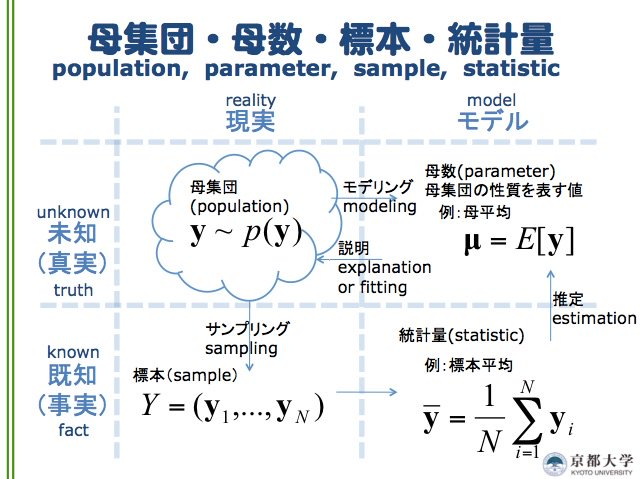
\includegraphics[width=15cm]{images/statistics_map.jpeg}
        \caption{統計学の体系(hogeより引用)}
    \end{center}
\end{figure}

\section{記述統計,推測統計の基本フロー}

統計学の手法を用いてデータを分析するとき,必ず「何のために統計学を用いるのか」という目的が設定されている(設定すべきである).闇雲に用いるのではなく,問題設定 -> 必要なデータの取得 -> データの解釈,という手順が踏まれるべきである.

問題設定には例えば以下のようなものが考えられる.

\begin{itemize}
    \item ある現象のデータからその傾向を見たい(記述統計)
    \item この仮説を検証したい(記述統計,推測統計)
    \item 手元のデータから未来のデータを予測したい(推測統計)
\end{itemize}

上記を踏まえ,記述統計,推測統計を行う際の基本的な流れをざっくりまとめてみる.両者の最終的なアウトプットの違いに着目すると良い.

\vspace{10pt}

\fbox{\parbox{\textwidth}{記述統計の流れ
    \begin{enumerate}
        \item 問題設定,必要なデータを決める
        \item データの取得
        \item データの要約
        \item データの解釈
    \end{enumerate}
    }
}

\vspace{10pt}

\fbox{\parbox{\textwidth}{推測統計の流れ
    \begin{enumerate}
        \item 問題設定(母集団の設定),必要なデータを決める
        \item データの取得
        \item データから母集団の性質に当てはまる数理モデルを構築
        \item 数理モデルを使った推定・推測・推論(データを生成する未知の真の確率分布)
        \item :数理モデルを使った推定・推測・推論の妥当性を考察
    \end{enumerate}
    }
}
\vspace{10pt}

\begin{itemize}
    \item 記述統計のアウトプット:対象となる現象,集団の性質,特徴の説明,解釈
    \item 推測統計のアウトプット:対象となる現象,集団の性質,特徴の予測.例えば,予測を行うための数理モデルがアウトプットになる.予測の検証まで行って初めて意味を成す.
\end{itemize}


注意点として,特に推測統計においては,上記の流れは上から下に綺麗に流れていくものではなく,上記の手順(例えば 2 ~ 4)を回すイメージである.

例えば、データが運悪く偏ってしまったせいで、統計分析の結果が真実からかけ離れてしまうリスクを考える。

\section{補足 データの解釈:定性的と定量的}

統計学,または統計学だけでなくもっと広い意味で「データに対する解釈」を行う際に,解釈の結果として何らか(統計学で使われる指標など)の数値に落とし込むことが当たり前のように感じられるが,必ずしも数値に落とし込むことだけが「データに対する解釈」ではない\footnote{現実に統計学が使われる場面(データ分析など)では,アウトプットとして何らかの数値(指標)に落とし込むことが求められるのがほとんどだとは思いますが...}.

データに対する特徴・性質を「言葉」で表すことも
